%!TEX TS-program = xelatex
%!TEX encoding = UTF-8 Unicode
\documentclass[12pt, xcolor=dvipsnames]{beamer}
\definecolor{slight}{gray}{0.9}
\fboxsep=10pt
\usecolortheme[named=Royal Blue]{structure}
\useinnertheme{circles}
\usepackage[no-math]{fontspec}
\usepackage{xltxtra, xunicode}
\usepackage[utf8]{inputenc}
%\usepackage[sc, osf]{mathpazo}
\usepackage[minionint, lf, mathtabular]{MinionPro}
\setmainfont[Mapping=tex-text]{Minion Web Pro}
\setsansfont[Mapping=tex-text]{Myriad Web Pro}
\setmonofont[Scale=MatchLowercase]{Source Code Pro}
\usefonttheme{professionalfonts}
%% 中文字配置
\usepackage[
CJKmath=true, indentfirst=false, PunctStyle={quanjiao},
CheckSingle=true, SlantFont, BoldFont
]{xeCJK}
\setCJKmainfont[Scale=0.9, BoldFont=Hiragino Mincho ProN W6]{Hiragino Mincho ProN W3}
%\setCJKmainfont[Scale=0.9, BoldFont=Noto Sans CJK JP Bold]{Noto Sans CJK JP Medium}
\setCJKsansfont[Scale=0.9, BoldFont=Hiragino Sans W6]{Hiragino Sans W4}
%\setCJKsansfont[Scale=0.9, BoldFont=Hiragino Sans CNS W6]{Hiragino Sans CNS W3}
%\setCJKsansfont[Scale=0.9, BoldFont=Hiragino Sans W7]{Hiragino Sans W4}
%\setCJKsansfont[Scale=0.9, BoldFont=Source Han Sans UI TC Bold]{Source Han Sans UI TC Regular}
%\setCJKsansfont[Scale=0.9, BoldFont=PingFang TC Semibold]{PingFang TC Regular}
\setCJKmonofont[Scale=0.9, BoldFont=Yuanti TC Regular]{Hiragino Maru Gothic ProN W4}
\usepackage{fancyvrb, attachfile2, pstricks}
\usepackage{graphicx}
\setbeamerfont{page number in head/foot}{size=\tiny}
\setbeamertemplate{footline}[frame number]
\usepackage{xmpmulti, booktabs, multicol}
\setbeamertemplate{navigation symbols}{}
\let\WriteBookmarks\relax
\usepackage{dcolumn}
\newcolumntype{.}[1]{D{.}{.}{#1}}
\newcolumntype{,}[1]{D{,}{,}{#1}}

\linespread{1.25}

\setbeamersize{text margin left=.8em, text margin right=.6em}

\makeatletter
\defbeamertemplate{itemize item}{mycircle}{\LARGE\raise-1.6pt\hbox{\textbullet}}
\makeatother

\setbeamertemplate{itemize item}[mycircle]
\setbeamertemplate{itemize subitem}[triangle]
\setlength\leftmargini{1.3em}
\setlength\leftmarginii{1em}


%\CTXFR
\title{\bf{\Huge {}\\[-2mm] Principles of Economics \\[2mm] Review Session}}
\author{{\Large 張耕齊\\[2mm] Keng-Chi Chang}}
\institute{{}\\[-7mm]\footnotesize\tt{<r03323070@ntu.edu.tw>}\\[2mm]}
\date{\large 2016.11.09}
\begin{document}
\fontsize{12}{14pt}\selectfont

\begin{frame}
\titlepage
\end{frame}

\begin{frame}
\frametitle{\bf Chapter 8: Trade}
\begin{itemize}
\item Everyone has at least one comparative advantage
\item By specializing your comparative advantage and exchange make the trade unit as a whole better off
\item Here we assume ``small country'' for simplicity, that is, countries take world price as given, hence the horizontal world price
\item Redistributions between sectors may occur
\item Tariffs make the society as a whole worse off
\end{itemize}
\end{frame}


\begin{frame}
\frametitle{\bf Pre-Trade: Autarky}
\begin{center}
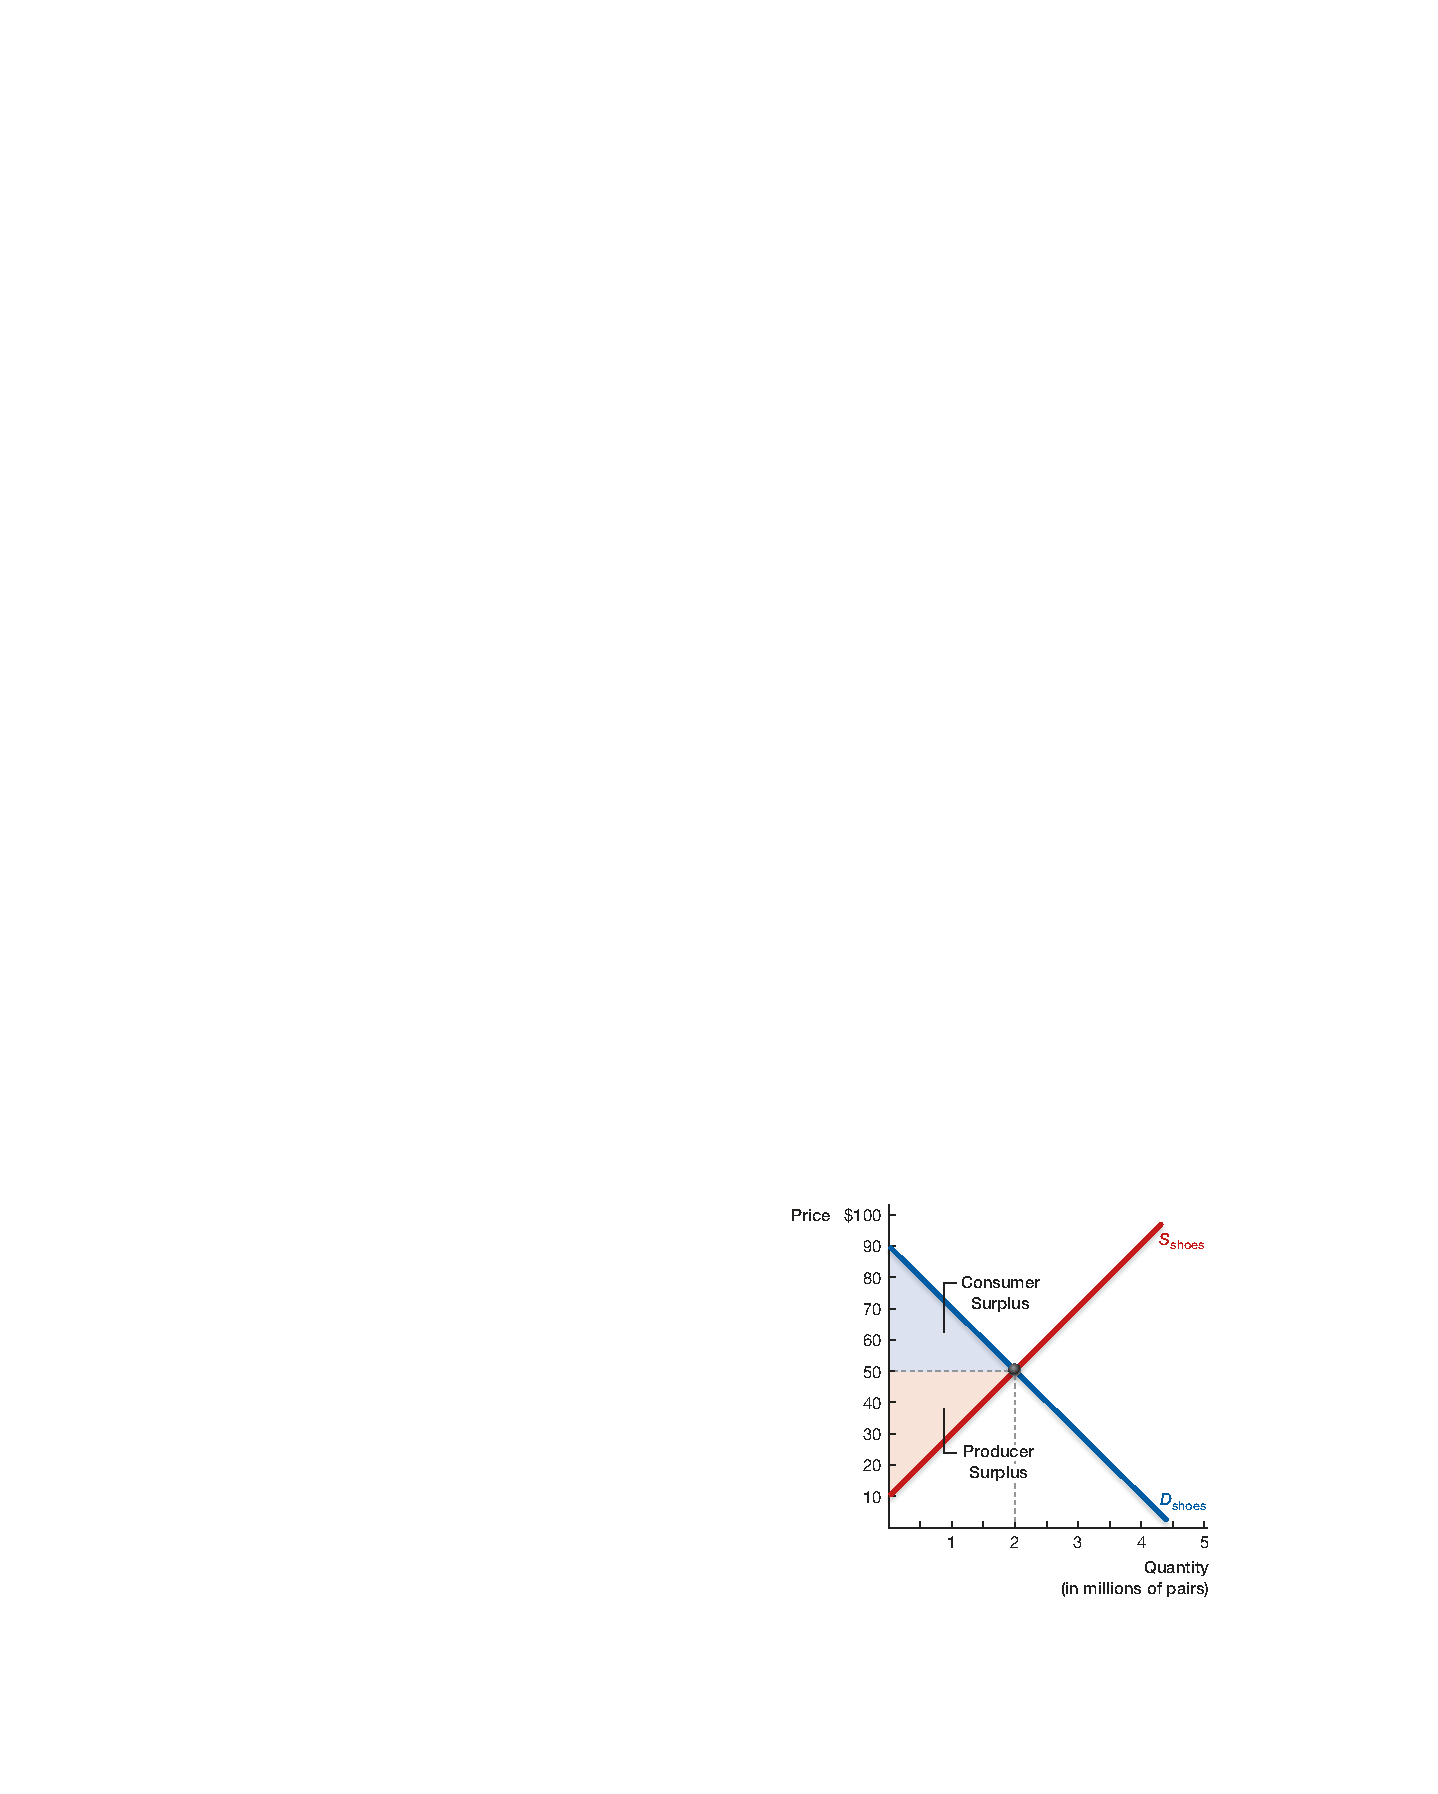
\includegraphics[height=.85\textheight]{figures/1.pdf}
\end{center}
\end{frame}


\begin{frame}
\frametitle{\bf Export Benefits Producers}
\begin{center}
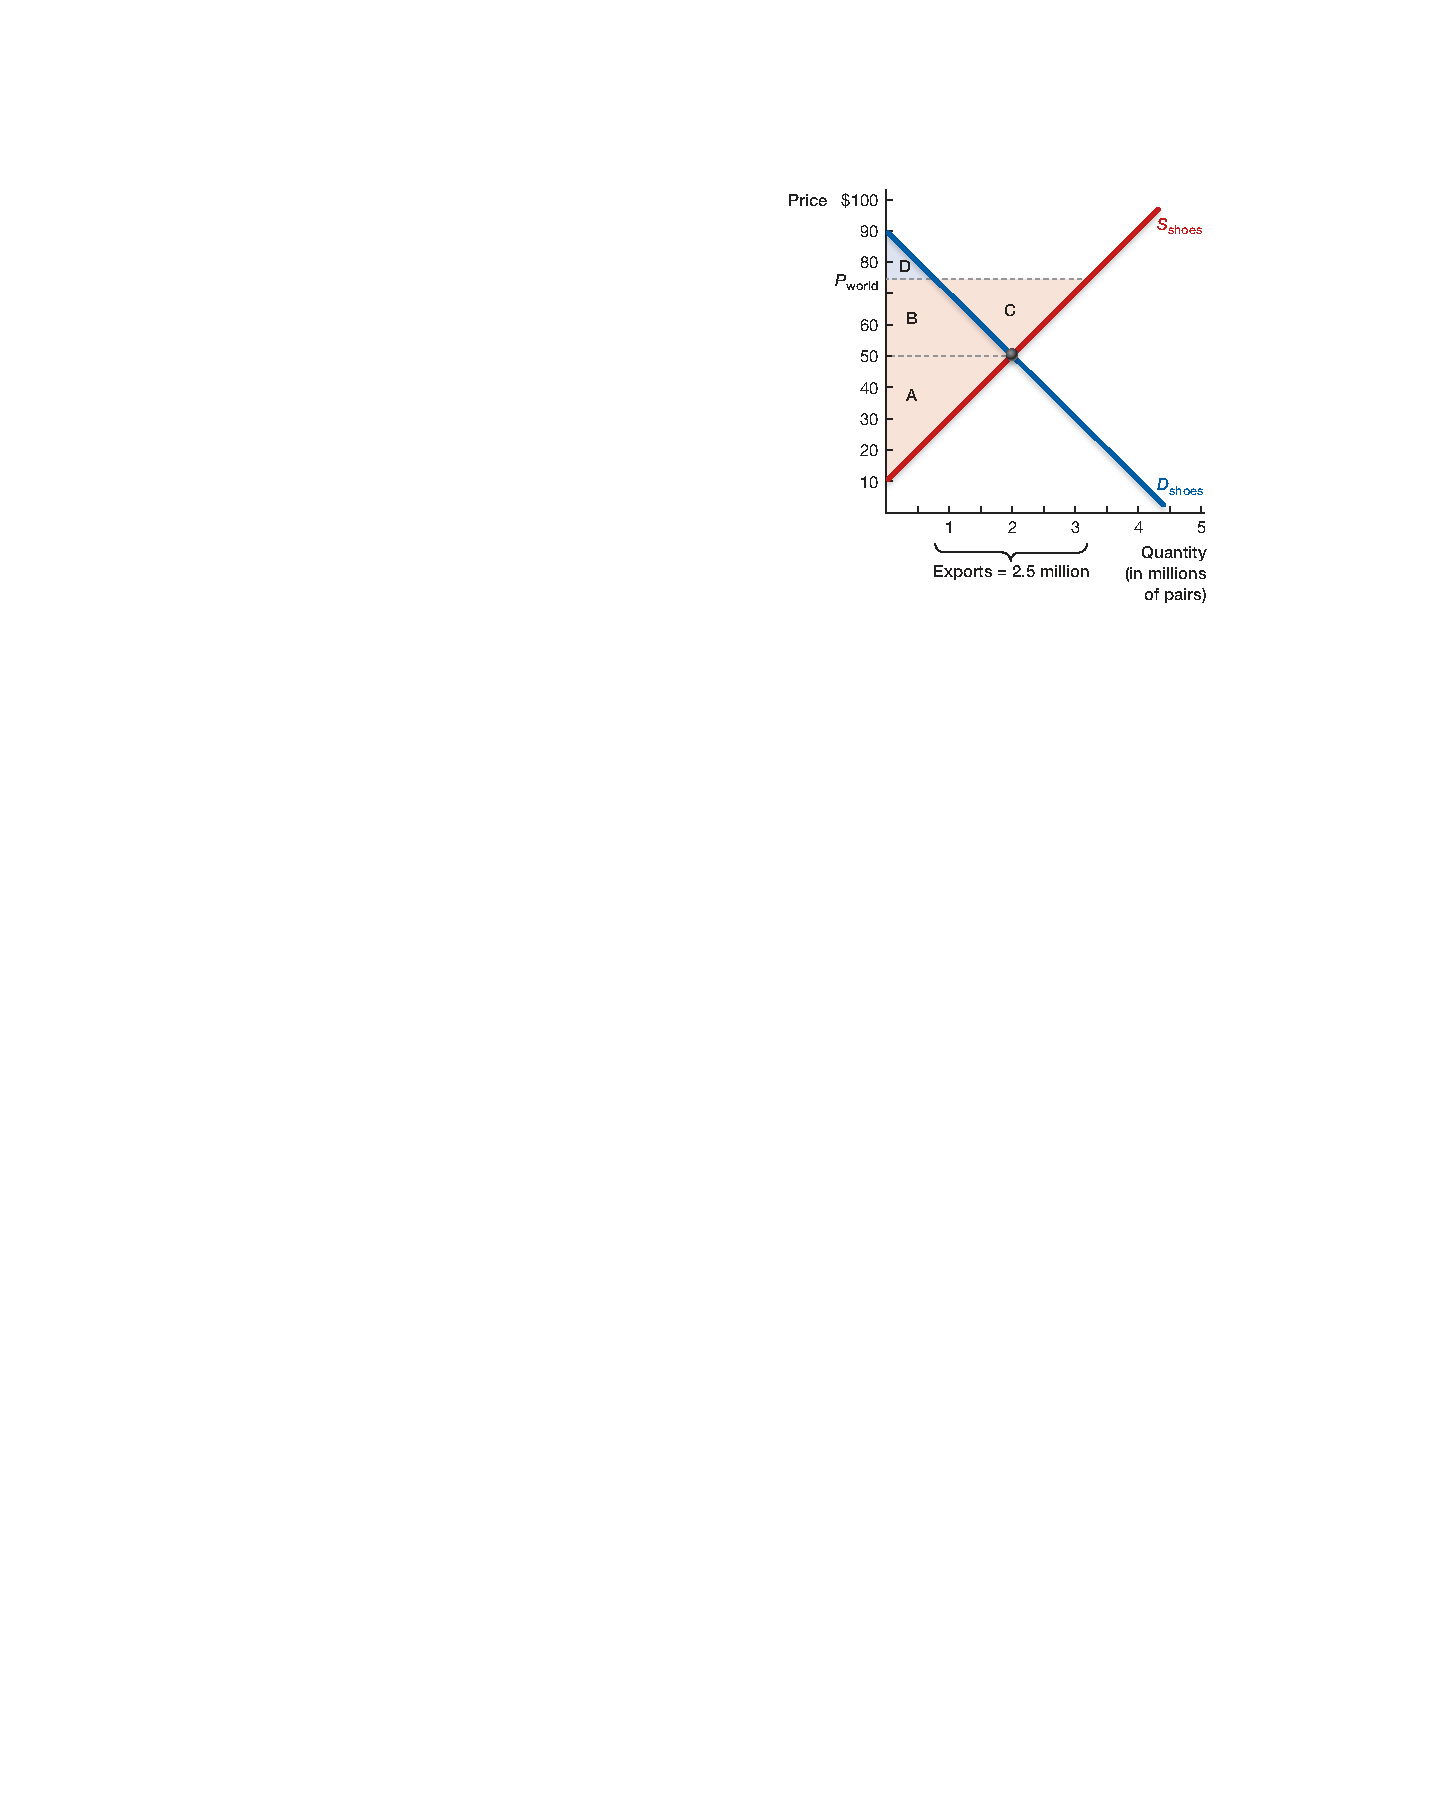
\includegraphics[height=.85\textheight]{figures/2.pdf}
\end{center}
\end{frame}

\begin{frame}
\frametitle{\bf Import Benefits Consumers}
\begin{center}
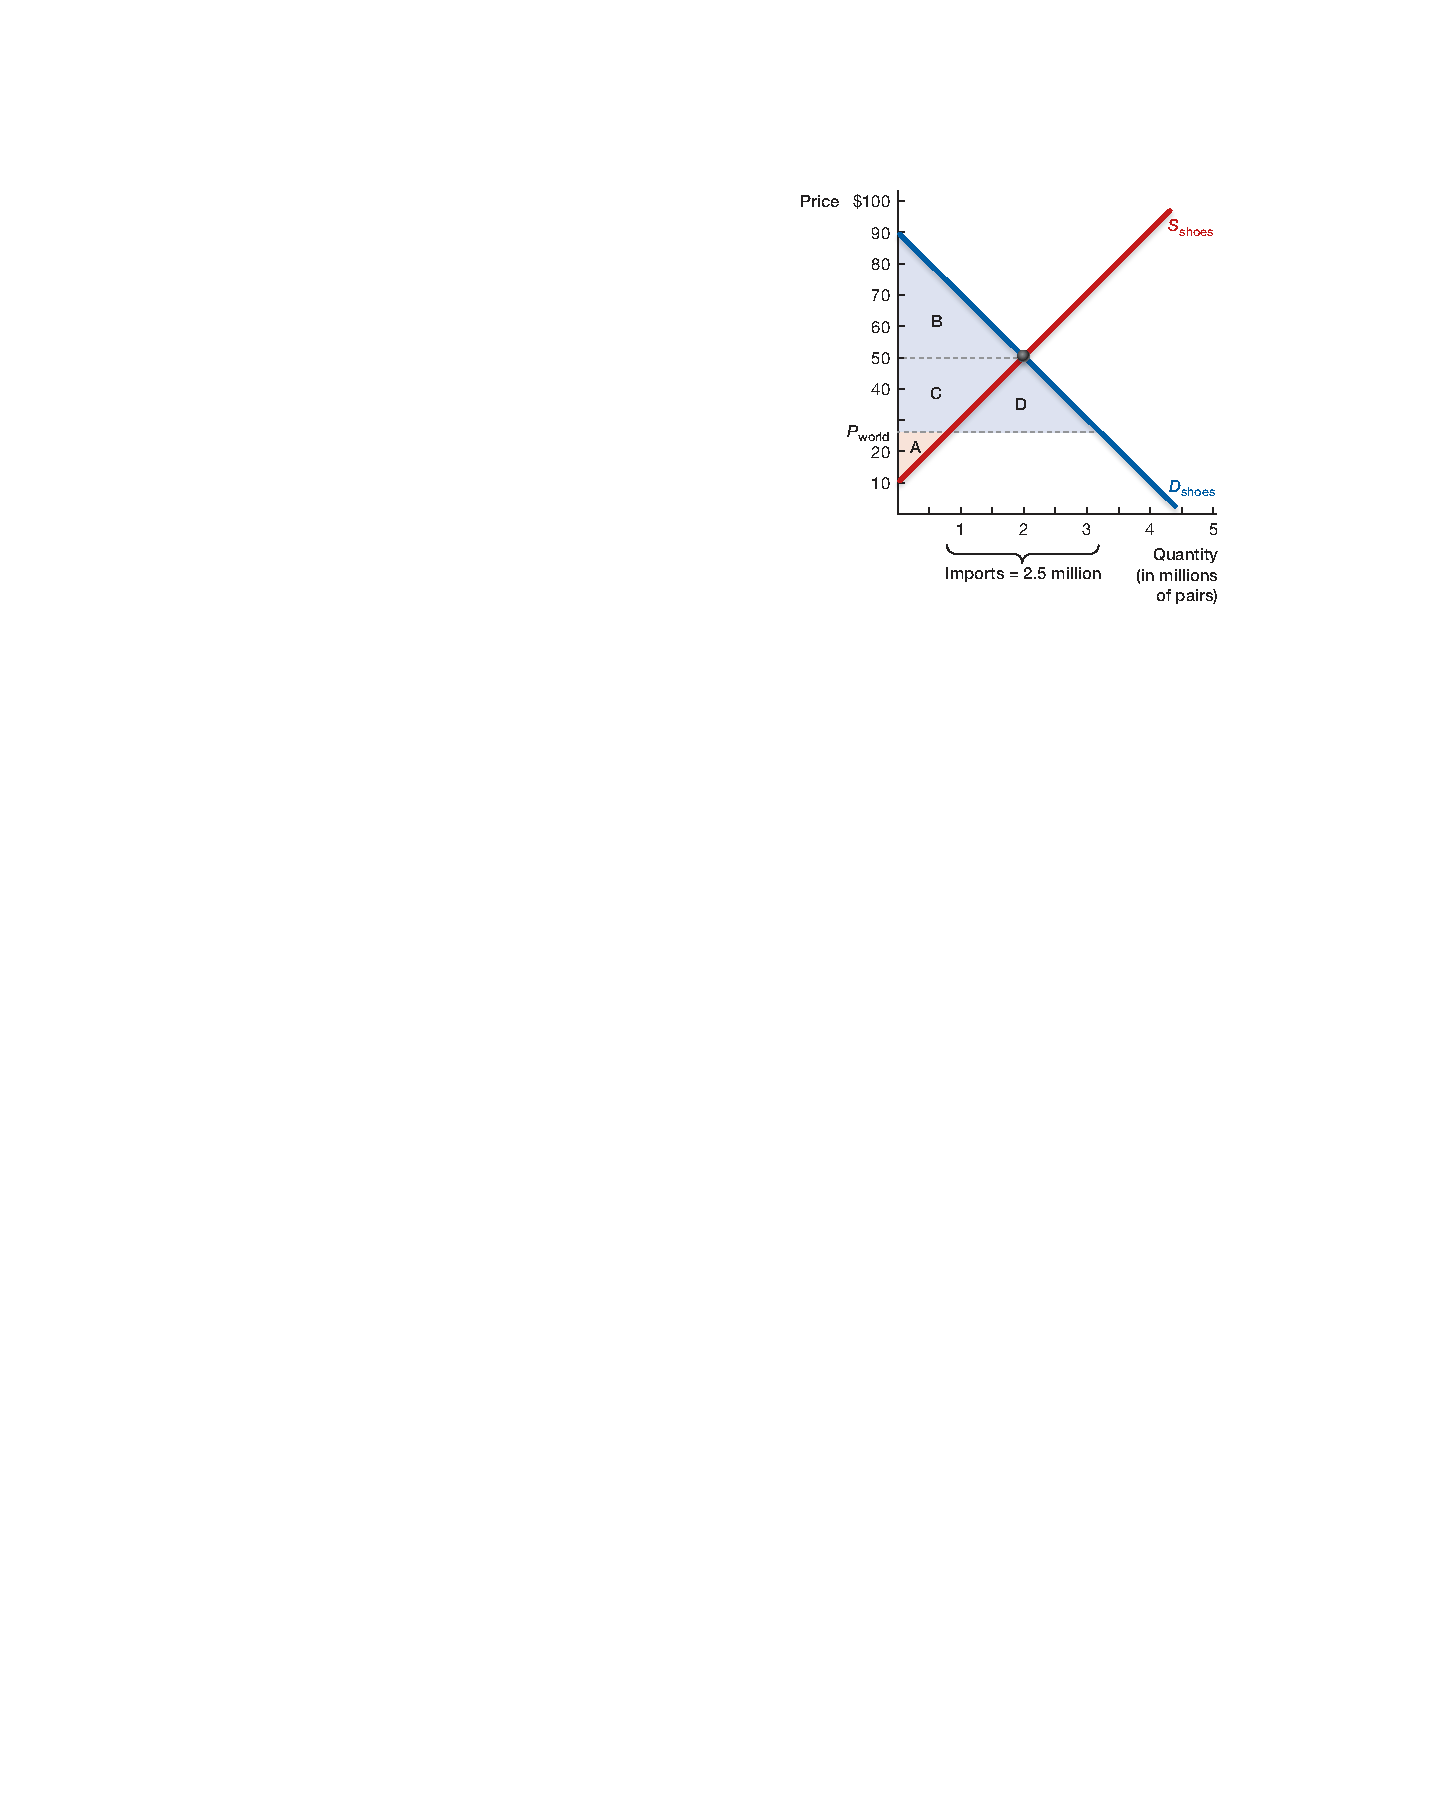
\includegraphics[height=.85\textheight]{figures/3.pdf}
\end{center}
\end{frame}

\begin{frame}
\frametitle{\bf Tariffs: Over-Produce and Under-Consume}
\begin{center}
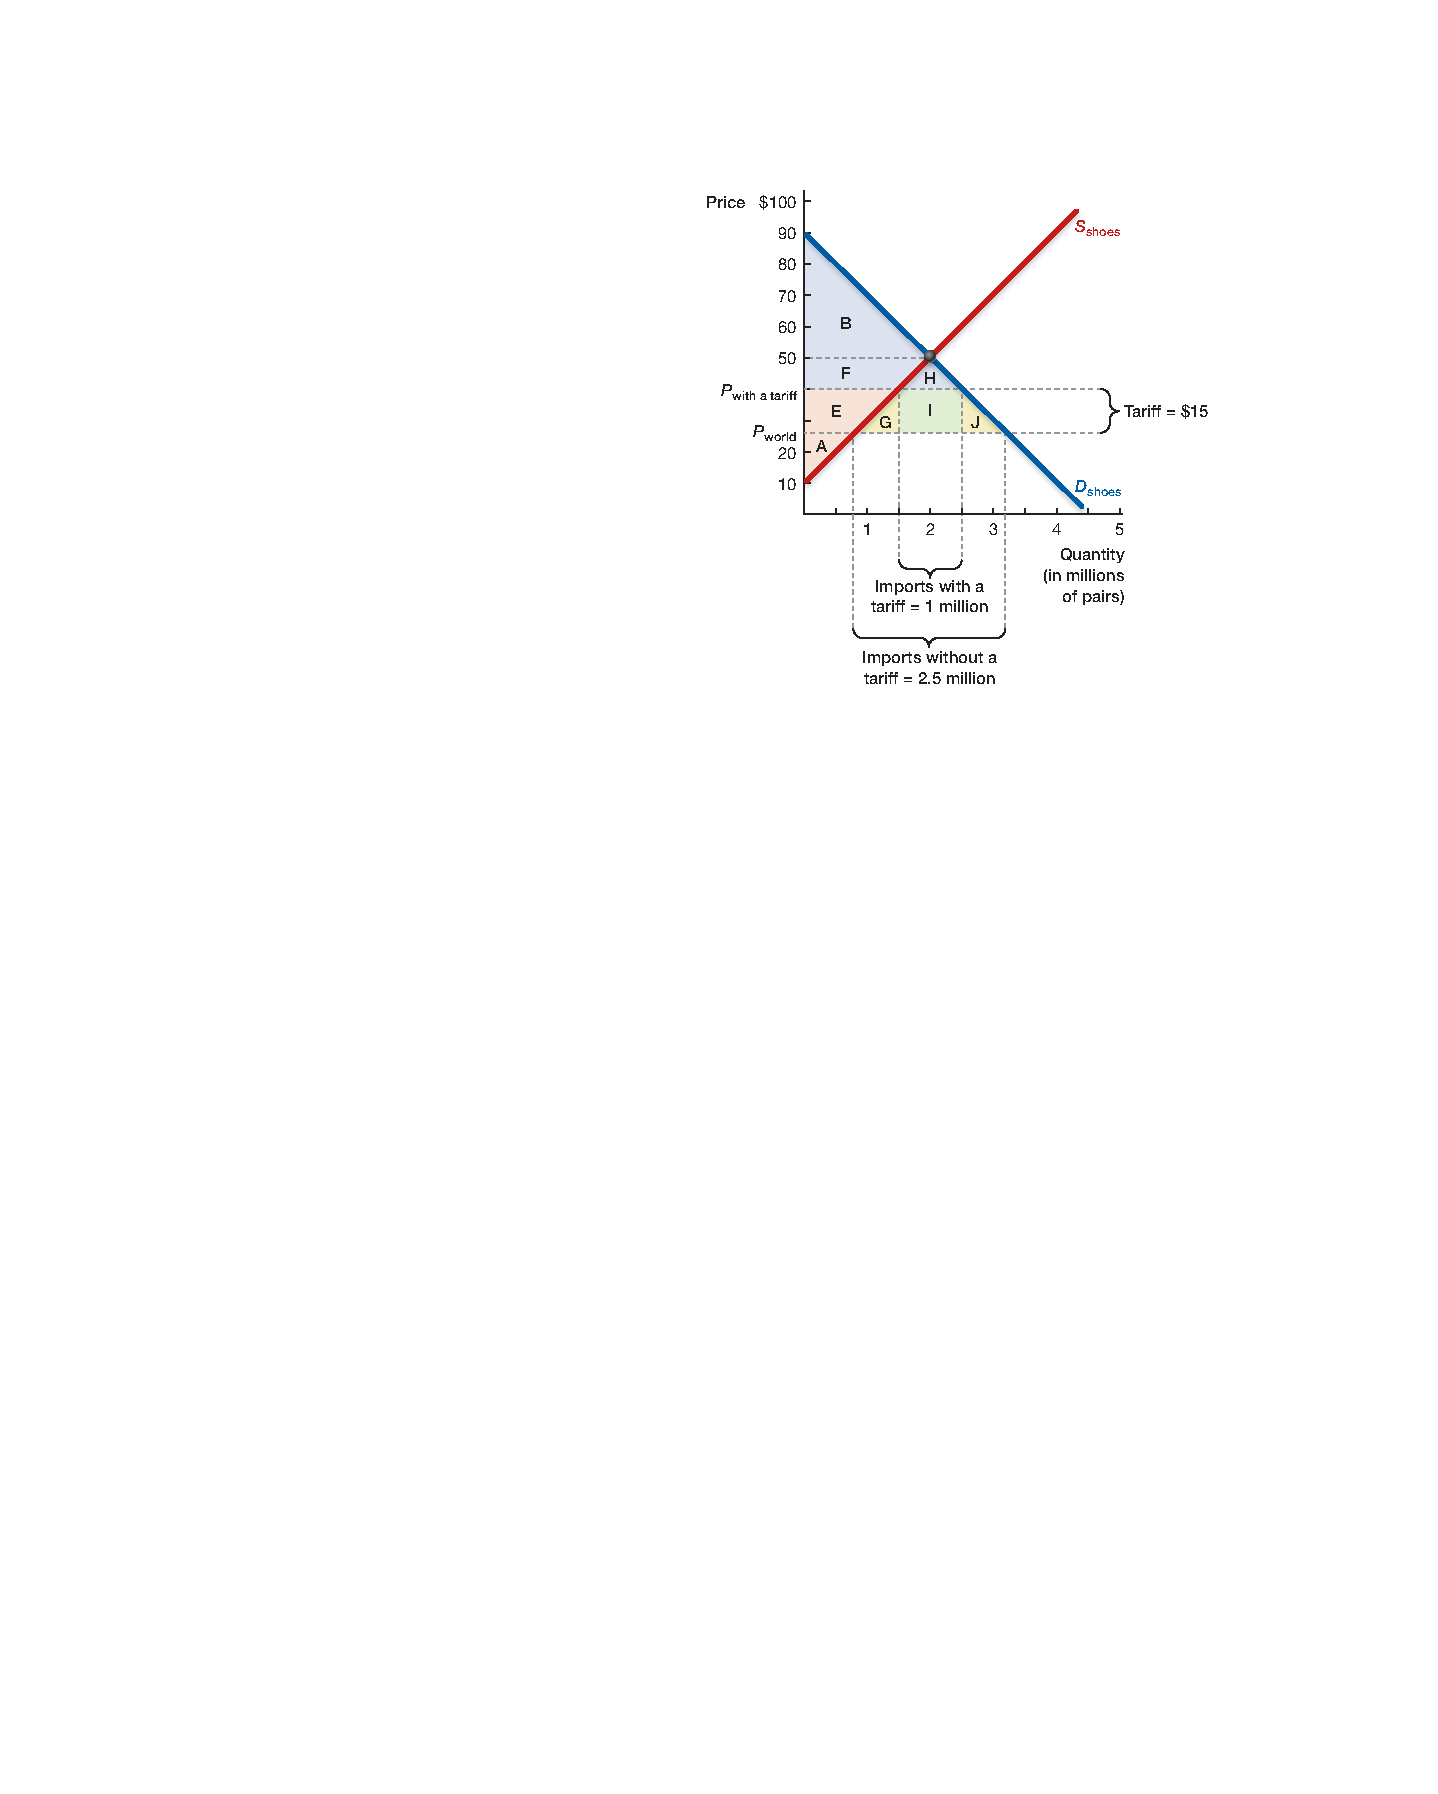
\includegraphics[height=.85\textheight]{figures/4.pdf}
\end{center}
\end{frame}

\begin{frame}
\frametitle{\bf §9.1--9.3: Externalities}
\begin{itemize}
\item Externalities are some costs or benefits not recognized by the buyers and sellers
\item This often creates over-produce or under-produce of goods, relative to the optimal quantity, so is inefficient
\item Possible solutions:
\begin{itemize}
\item Pigou: Internalizing the externalities, usually through tax
\item Coase: Define property rights and let people bargain
\end{itemize}
\item Coase Theorem: When property rights are clearly defined and if there is no transaction cost, private bargaining always achieves the efficient outcome. So the initial allocation of property rights do not matter.
\end{itemize}
\end{frame}

\begin{frame}
\frametitle{\bf Negative Production Externality}
\begin{center}
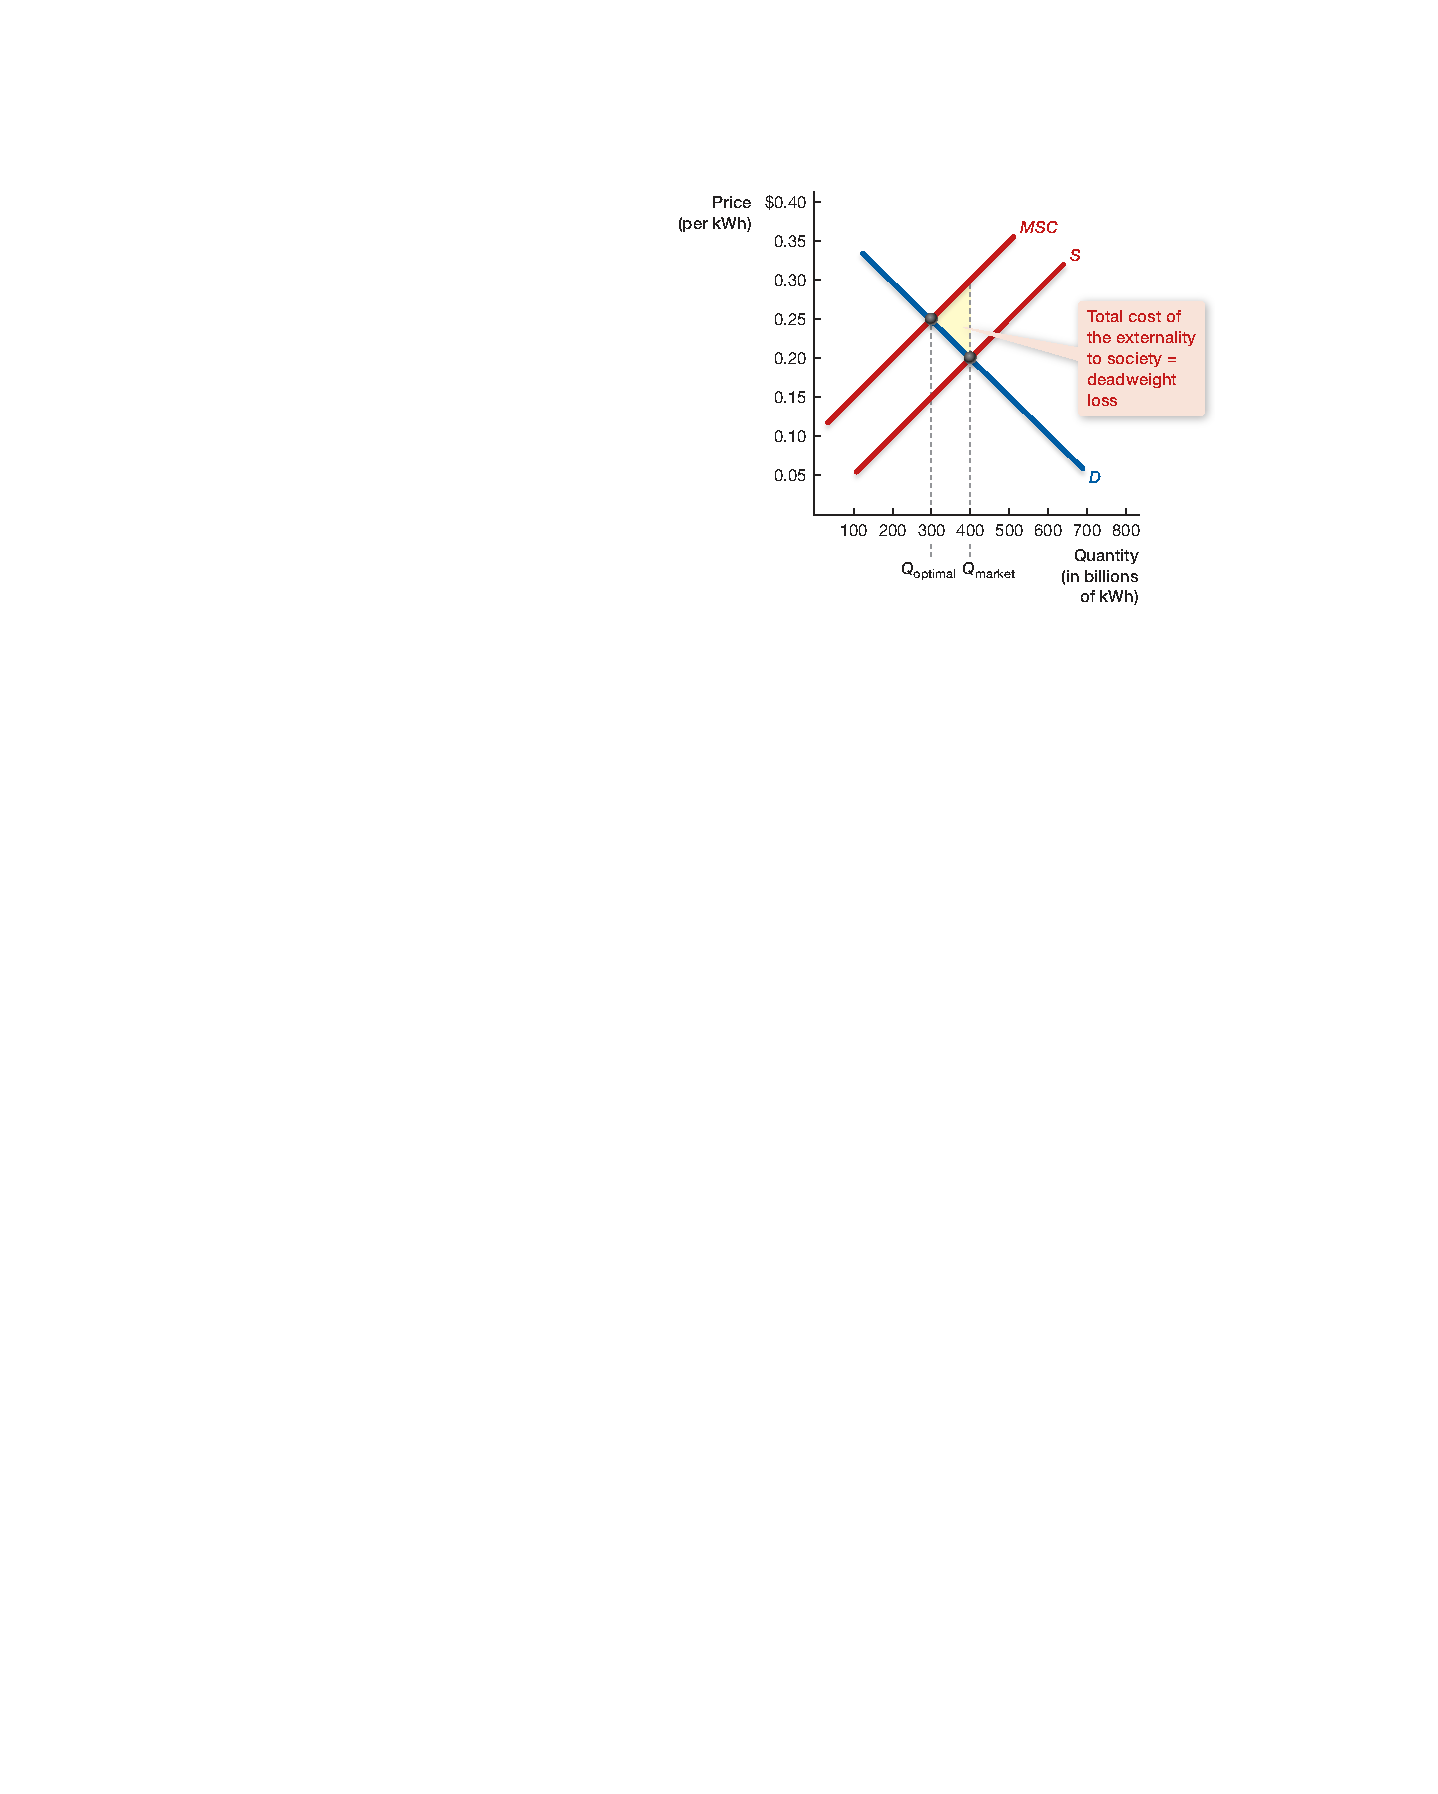
\includegraphics[height=.85\textheight]{figures/5.pdf}
\end{center}
\end{frame}

\begin{frame}
\frametitle{\bf Positive Consumption Externality}
\begin{center}
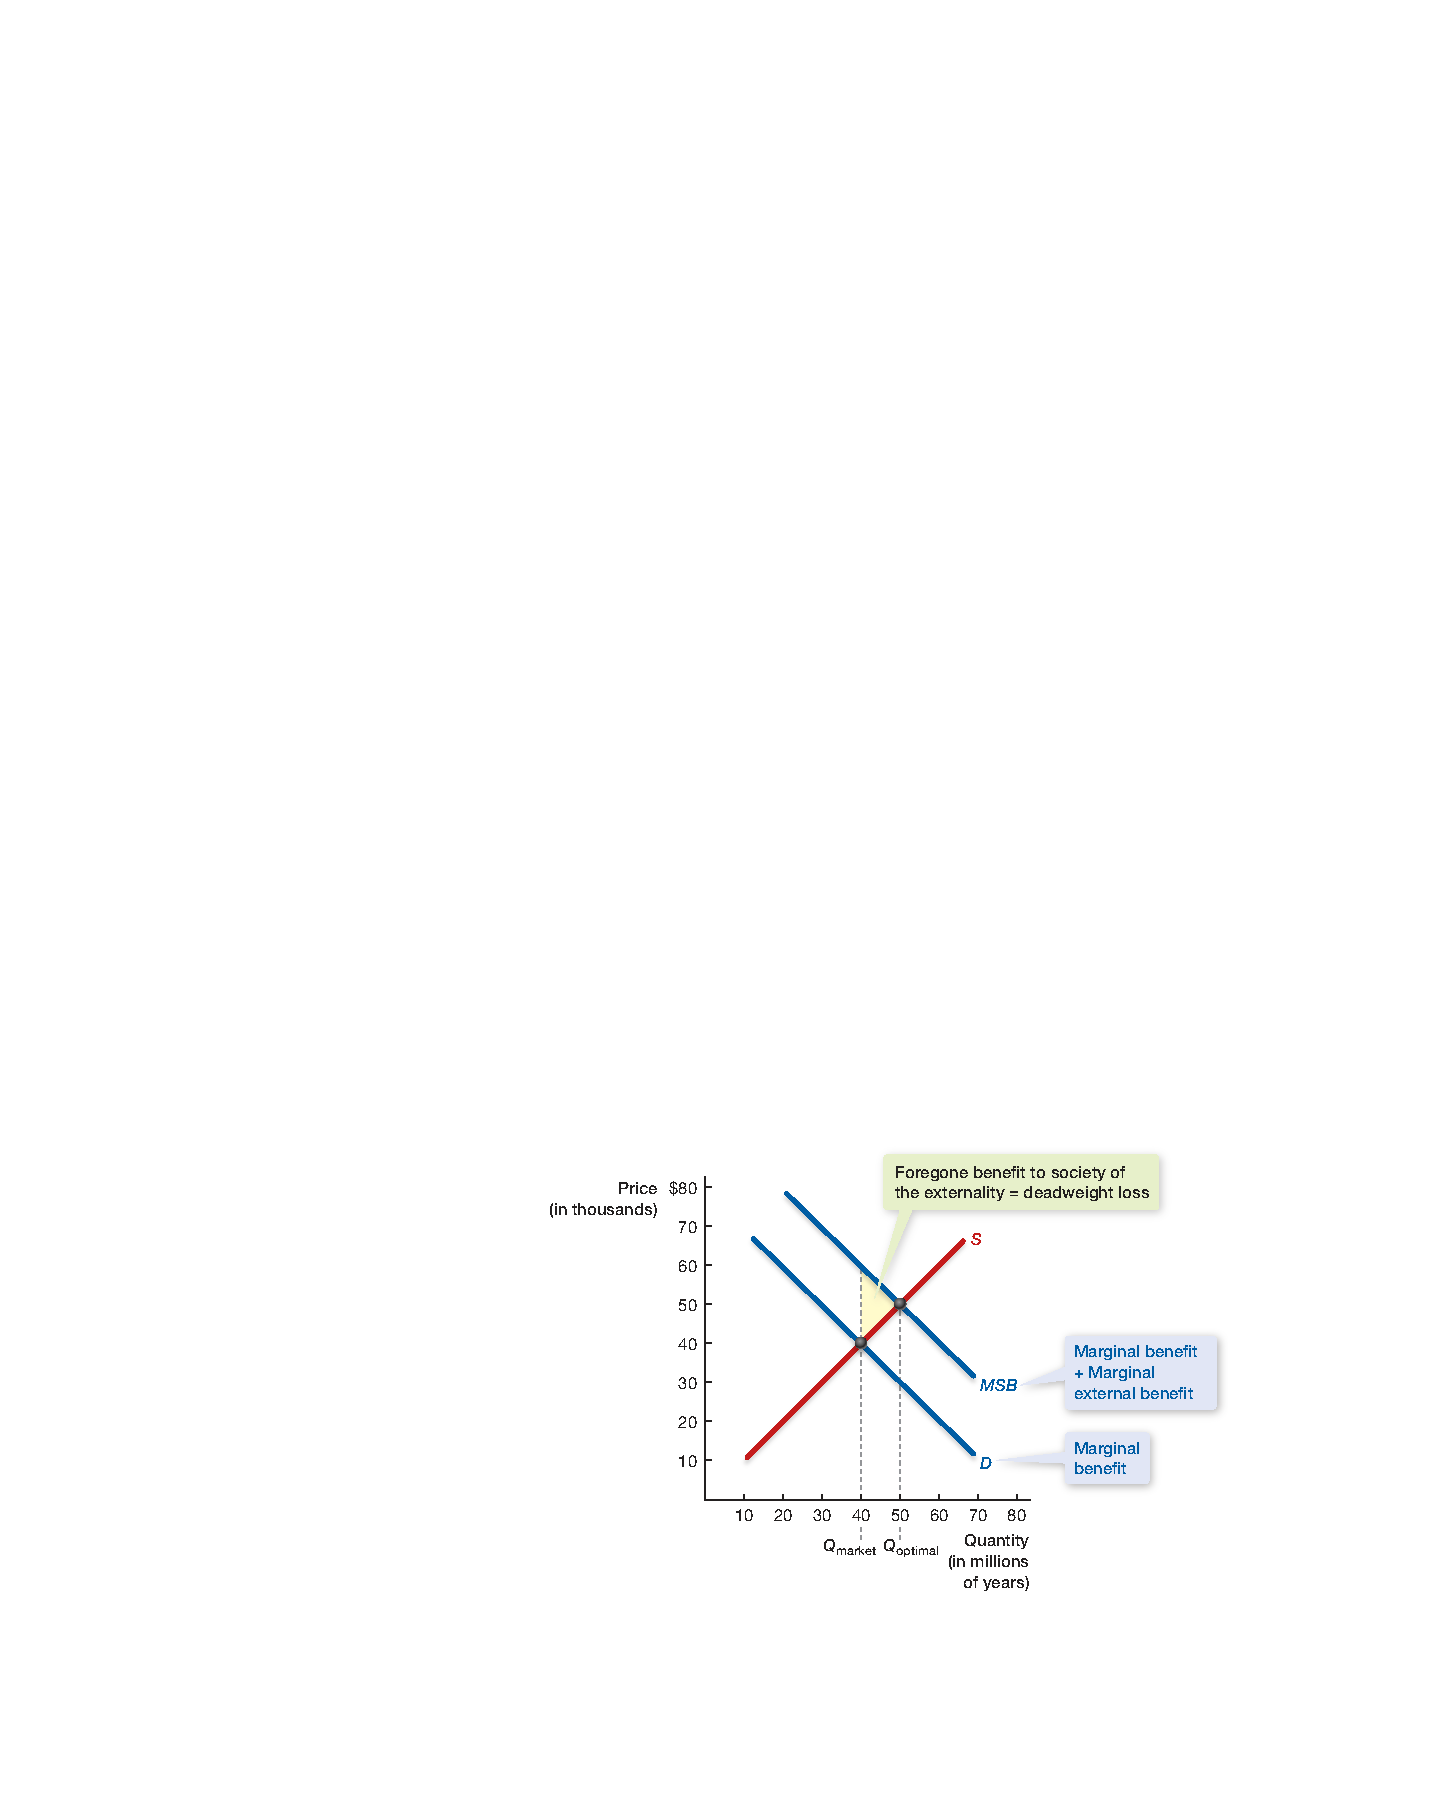
\includegraphics[height=.85\textheight]{figures/6.pdf}
\end{center}
\end{frame}

\begin{frame}
\frametitle{\large \bf §9.4--9.5: Public Goods and Common Resources}
\begin{itemize}
\item Public goods and common resources are both hard to exclude other people's usage
\item But common resources are rival in consumption, public goods are not
\item So we often see over-consumption of common resources (tragedy of commons)
\item And under-production of public goods (free-rider problem)
\end{itemize}
\end{frame}


\begin{frame}
\frametitle{\bf Chapter 10: Tax}
\begin{itemize}
\item Since quantity is no longer at the efficient level, taxtation usually creates deadweight loss
\item Tax incidence and equilibrium price and quantity after tax is independent of whom the tax is levied on
\item The more inelastic one is, the more tax burden one gets
\item Taxing inelastic goods will have fewer deadweight loss
\end{itemize}
\end{frame}

\begin{frame}
\frametitle{\bf Tax on Producers}
\begin{center}
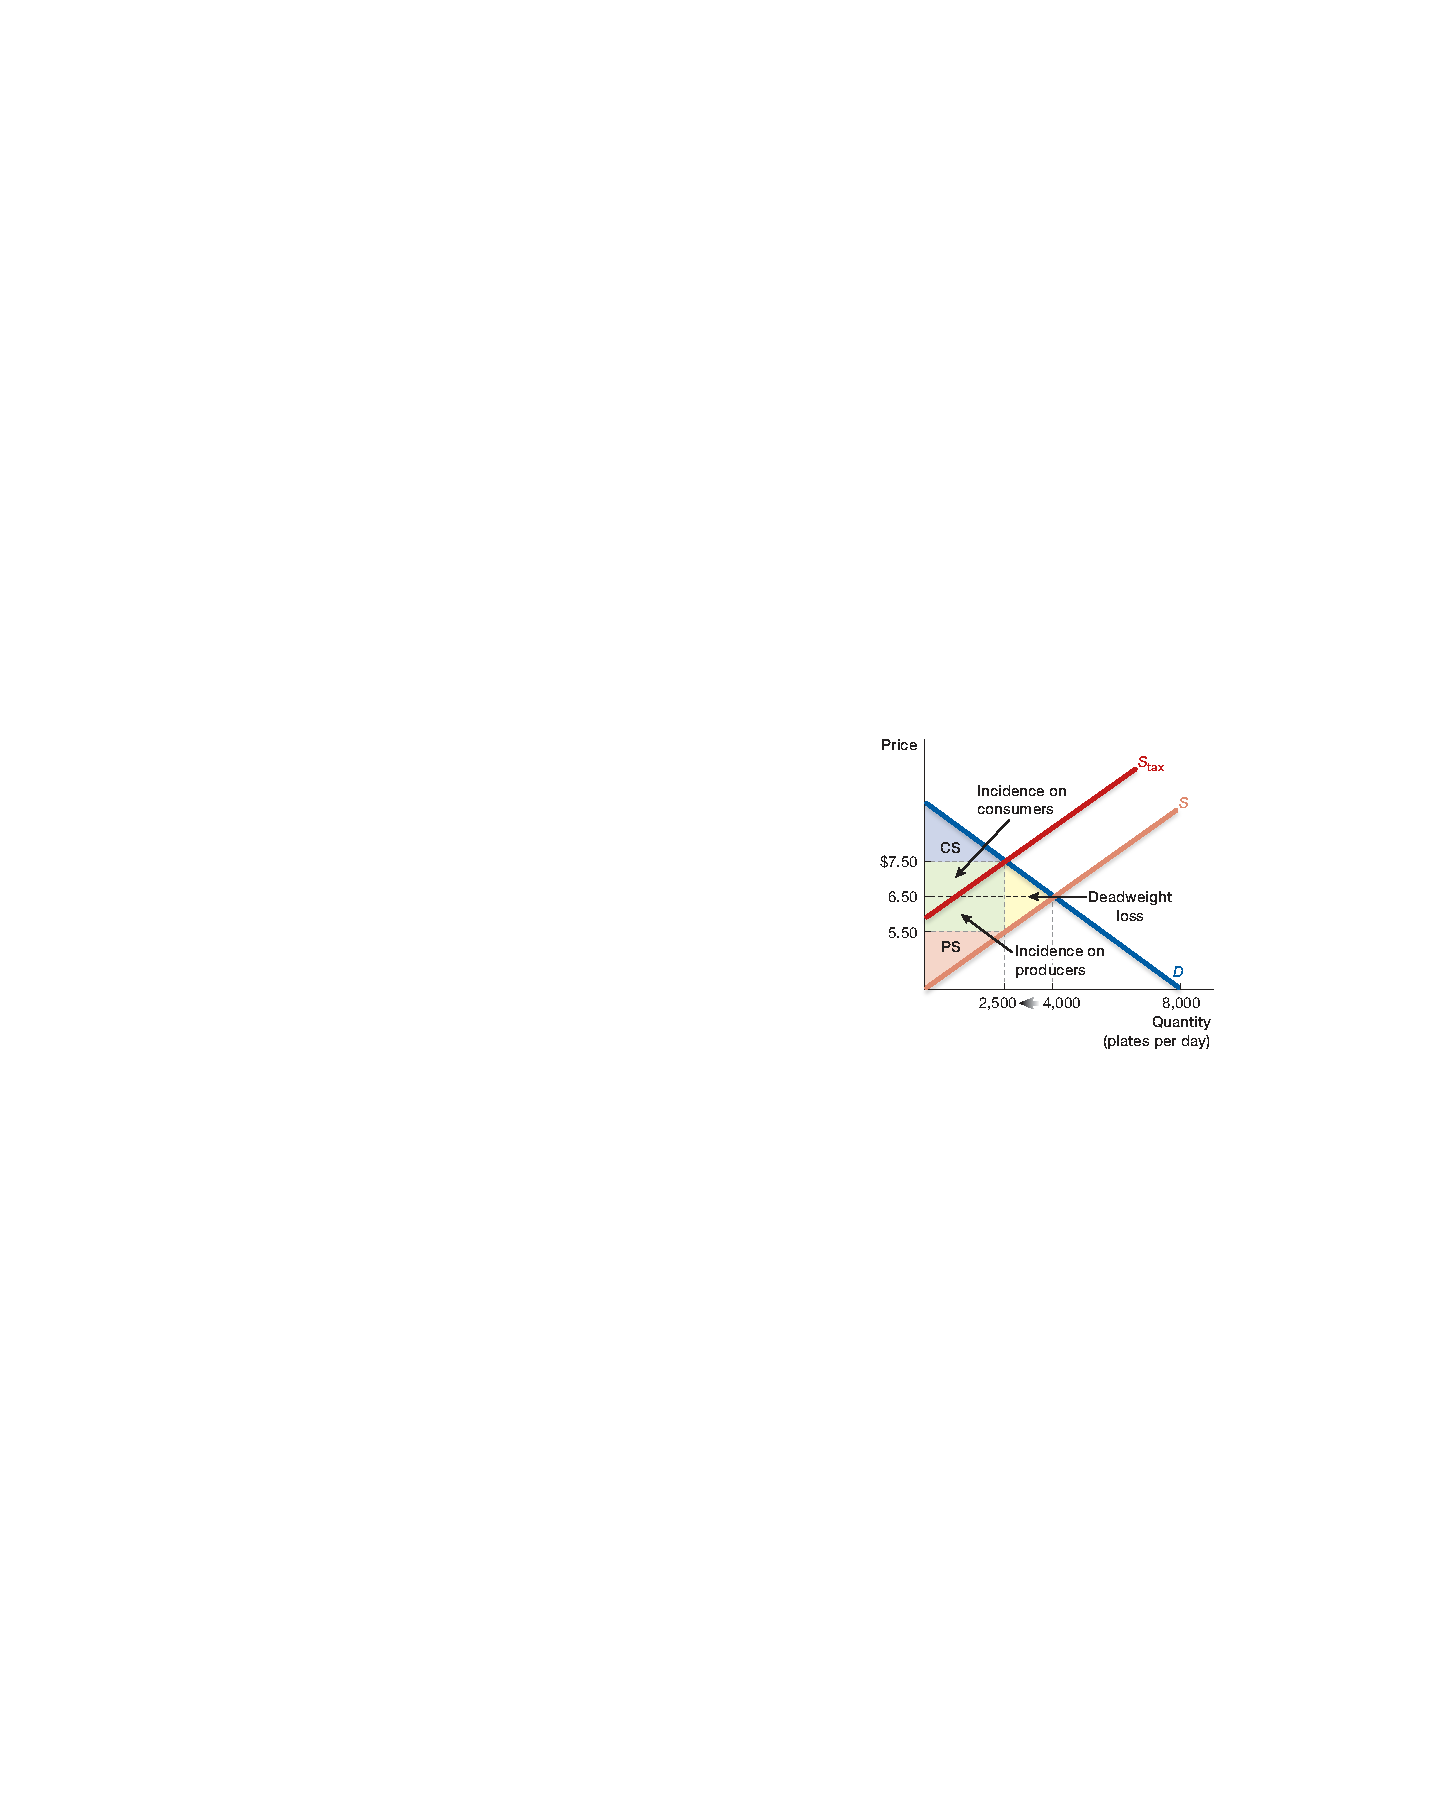
\includegraphics[height=.85\textheight]{figures/7.pdf}
\end{center}
\end{frame}


\begin{frame}
\frametitle{\bf Tax on Consumers}
\begin{center}
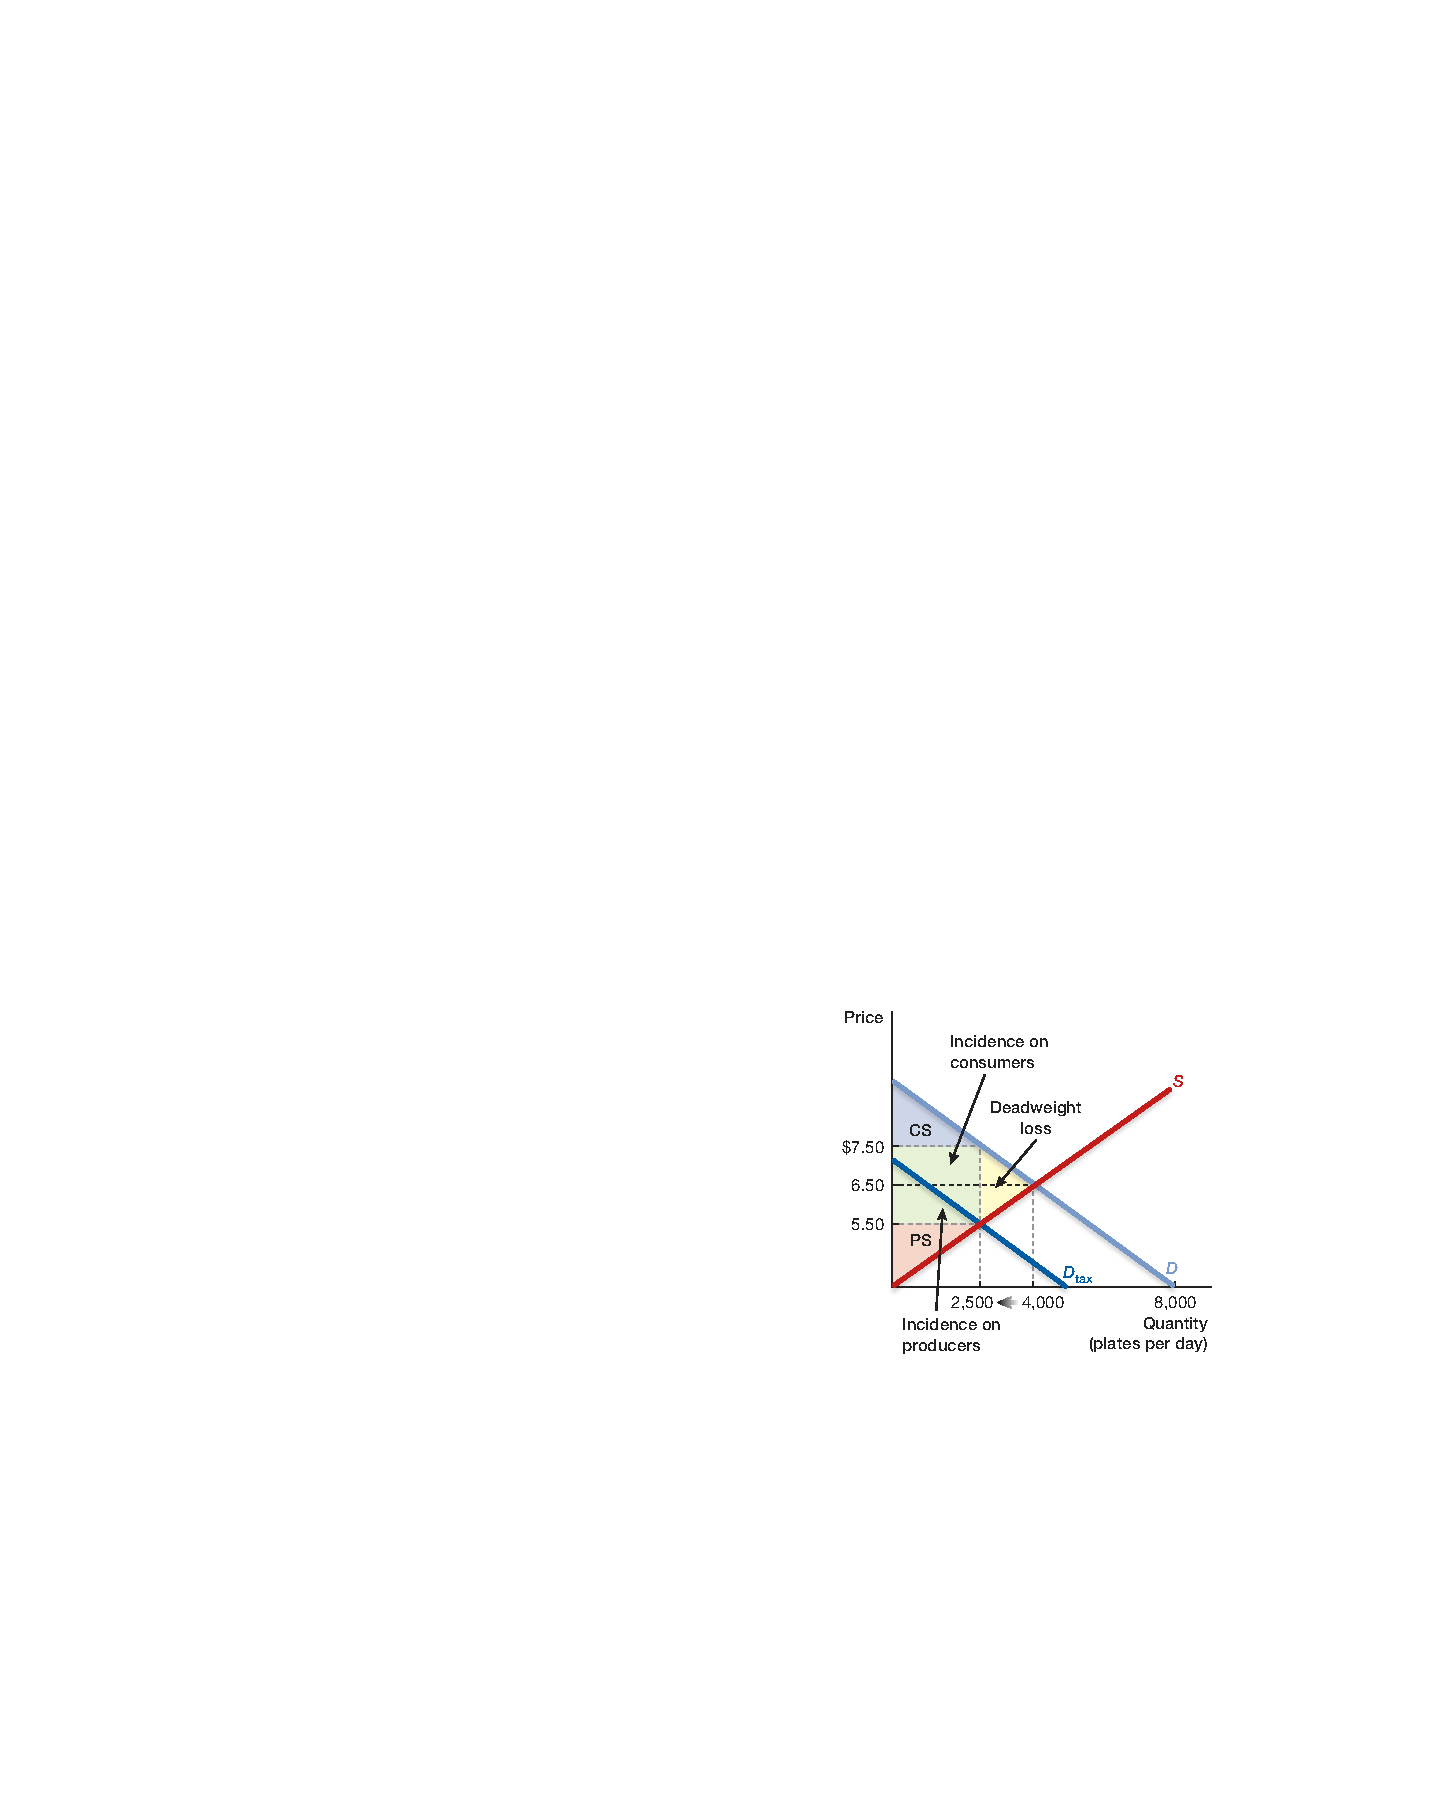
\includegraphics[height=.85\textheight]{figures/8.pdf}
\end{center}
\end{frame}


\begin{frame}
\frametitle{\bf More Elastic, Less Tax Burden}
\begin{center}
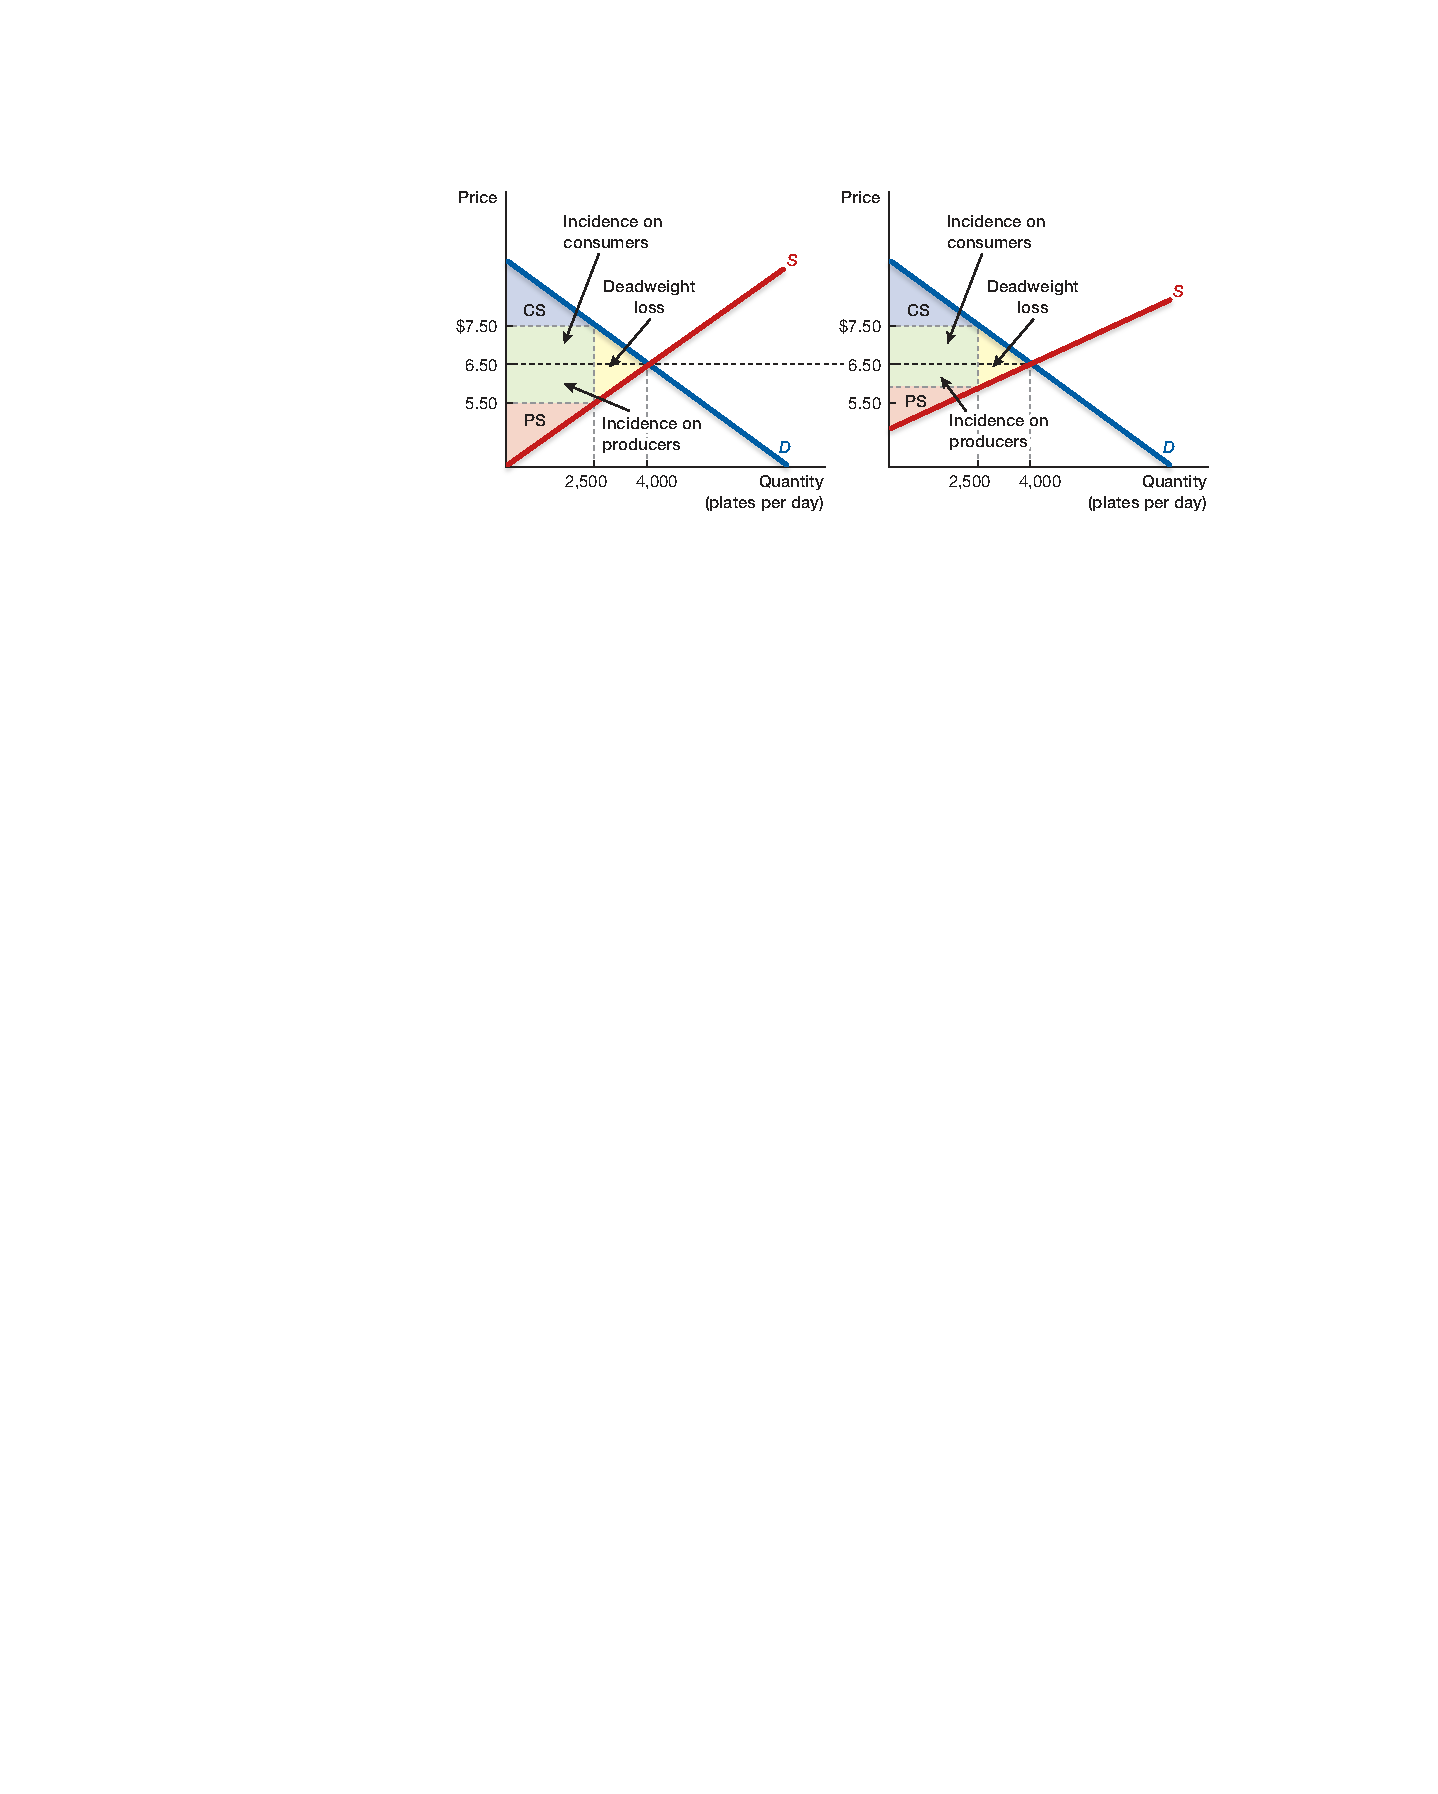
\includegraphics[width=\linewidth]{figures/9.pdf}
\end{center}
\end{frame}


\begin{frame}
\frametitle{\bf Tax, Deadweight Loss, and Elasticity}
\noindent \small \textsf{\bfseries Midterm 2008 Multiple Choice Q8.}
Suppose that policymakers are considering placing a tax on either of two markets. In Market A, the tax will have a significant effect on the price consumers pay, but it will not affect equilibrium quantity very much. In Market B, the same tax will have only a small effect on the price consumers pay, but it will have a large effect on the equilibrium quantity. Other factors are held constant. In which market will the tax have a larger deadweight loss?
\begin{enumerate}\itemsep-0.5ex
\item[A.] Market A
\item[B.] Market B
\item[C.] The deadweight loss will be the same in both markets.
\item[D.] There is not enough information to answer the question.
\end{enumerate}
\end{frame}



\begin{frame}
\frametitle{\bf Tax, Deadweight Loss, and Elasticity}
\noindent \small \textsf{\bfseries Midterm 2009 Multiple Choice Q15.}
Which of the following combinations will minimize the deadweight loss from a tax?
\begin{center}
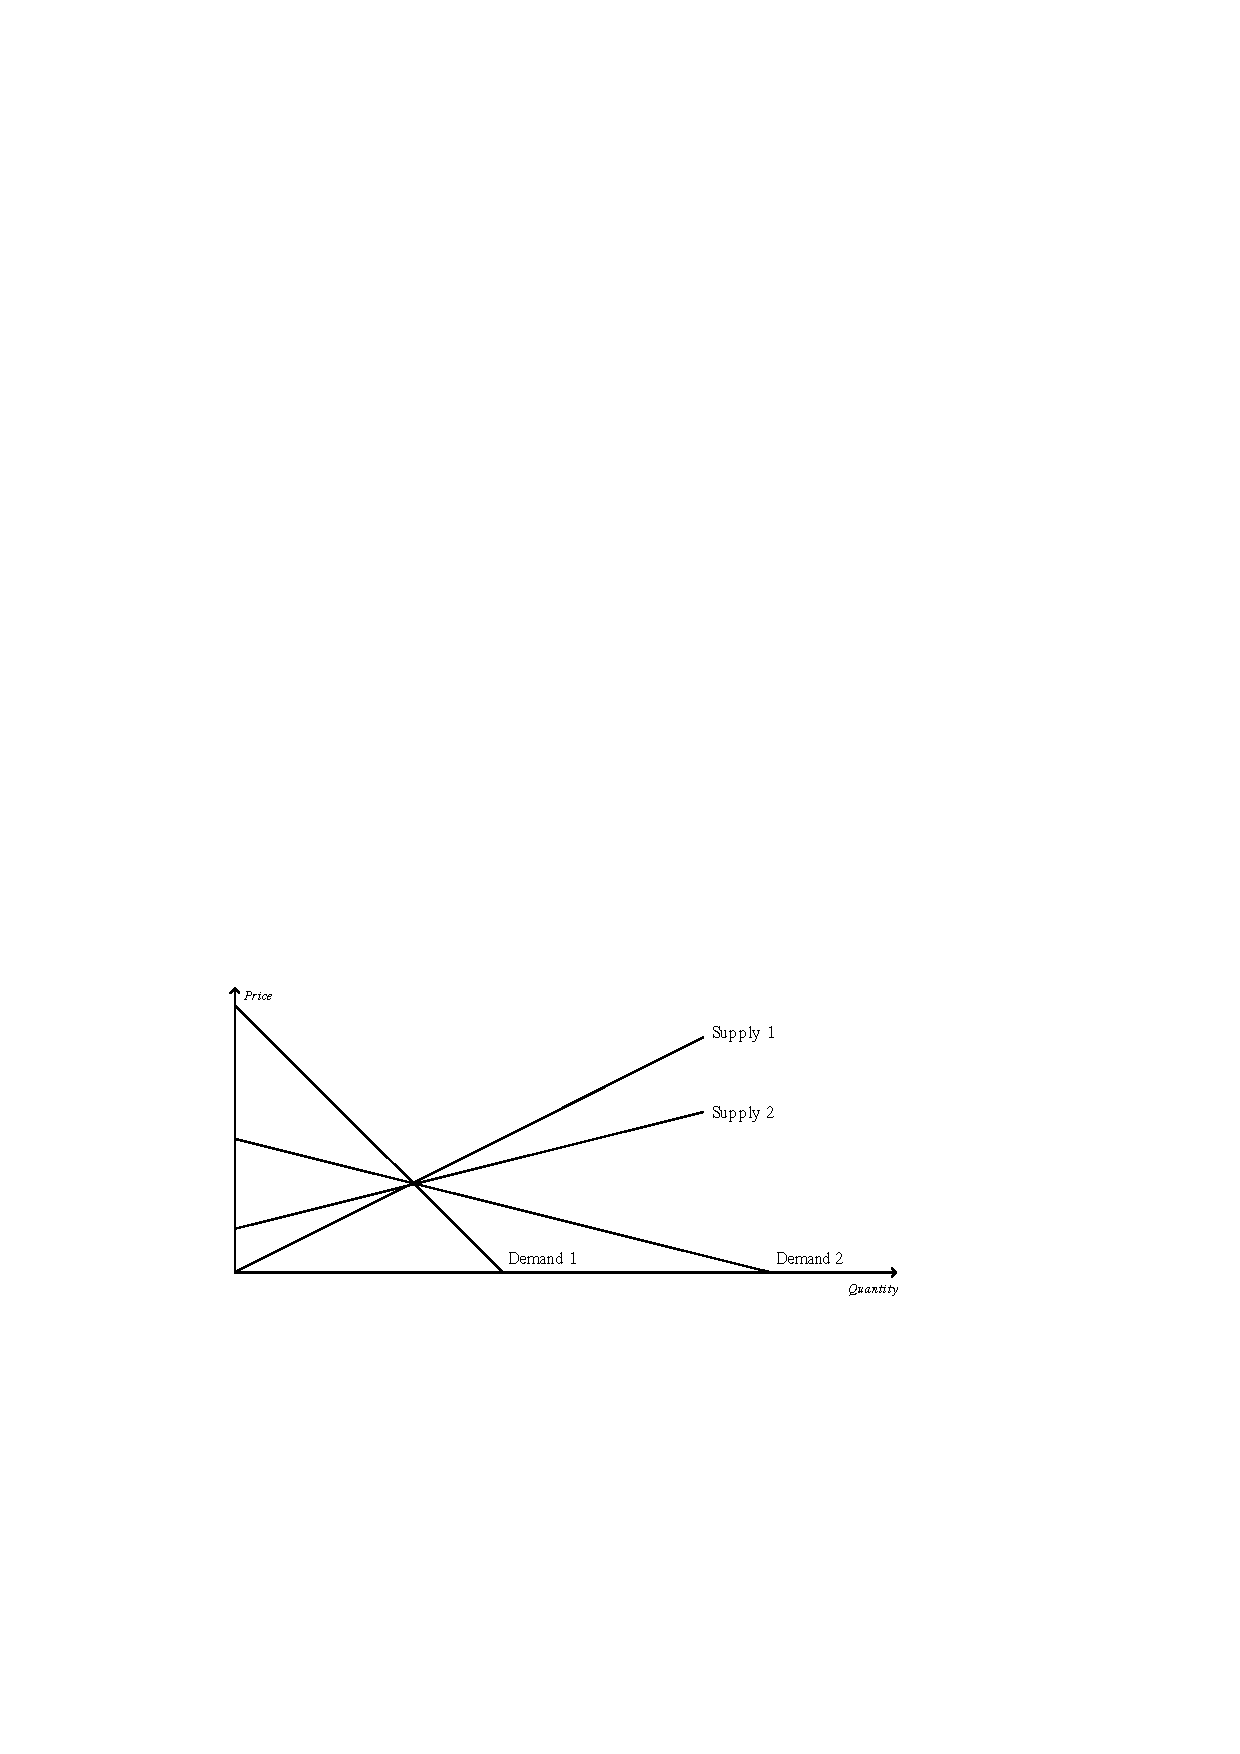
\includegraphics[width=\linewidth]{figures/10.pdf}
\end{center}
\end{frame}


\end{document}